\documentclass{llncs}
\pagestyle{plain}
\usepackage{graphicx}
\usepackage{hyperref}
\usepackage{amsmath,amssymb}
\usepackage{tabularx}
\usepackage{algorithm}
\usepackage{algpseudocode} 
\renewcommand{\algorithmicrequire}{\textbf{Input:}}
\renewcommand{\algorithmicensure}{\textbf{Output:}}
\usepackage{moreverb}
\usepackage[dvipsnames,table]{xcolor}
\usepackage[style=alphabetic,sorting=debug]{biblatex}

\DeclareFieldFormat{labelalpha}{\thefield{entrykey}}
\DeclareFieldFormat{extraalpha}{}
\addbibresource{sca,ANSSI}
\newtheorem{assumption}{Assumption}
\newenvironment{notation}{\begin{trivlist}\item[] {\em Notation.}}%
{\samepage \end{trivlist}}

% Probability definitions

\newcommand\myP[1]{\ensuremath\mathsf{P}\lbrack #1 \rbrack}     % The probability
\newcommand\myE[1]{\ensuremath\mathsf{E}\lbrack #1 \rbrack}     % The expectation
\newcommand\myV[1]{\ensuremath\mathsf{Var}\lbrack #1 \rbrack}   % The variance
\newcommand\mycov[2]{\ensuremath\mathsf{Cov}\lbrack #1;#2 \rbrack}   % The covariance
\newcommand\myI[2]{\ensuremath\mathsf{I}\lbrack #1;#2 \rbrack}  % The mutual information
\newcommand\myH[1]{\ensuremath\mathsf{H}\lbrack #1 \rbrack}     % The entropy
\newcommand\todo[1]{\textcolor{red}{TODO: #1}}
\newcommand{\codel}{$(3,6)\text{-code}$ }

% Finite Fields definitions

\def \GF {\mathrm{GF}}
\def \GFn {\GF(2^n)}
\def \GFm {\GF(2^m)}
\def \nbShares {n}
\def \order {d}
\newcommand{\pubEltNoIndex}[1][i]{\alpha}
\newcommand{\pubElt}[1][i]{\alpha_{#1}}
\newcommand{\pubEltStar}{\alpha^{\star}}
\newcommand{\polyCoef}[1][i]{u_{#1}}
\newcommand{\RS}[1][]{\mathrm{RS}(#1)}
\def \Field {\mathbb{K}}
\def \FField {\mathbb{F}}
\def \pubSet{\mathcal{S}}
\def \myTrace {\mathrm{tr}_{\Field/\FField}}
\def \polySet {\mathcal{P}(\pubEltStar)}

% Editorial definitions

\def\etal{\textit{et al.} }
\newcommand {\ie}{{\em i.e.} }
\def\eg{\textit{e.g.} }
\def\resp{{\em resp.} }
\def\myth{$^\text{th}$}

% ECC
\def\RSCode{\mathcal{C}}
\def\RSProduct{\mathcal{C}^{\star}}
\newcommand{\trans}[1][\RSProduct \rightarrow \RSCode] {\mathrm{\bf transcoding}_{#1}}
\def \wordRS {c}
\def \wordRSNew {\hat{c}}
\def \wordRSProduct {c^{\star}}
\def \wordRSProductZero {c^{0}}


% Comments
\def\comEP#1{\textcolor{RoyalPurple}{{\bf EP: #1}}}

\title{Enhancement of Shamir's Secret Sharing Schemes against Side-Channel Attacks}

\author{Anonymous submission to CHES'2017}
\institute{}

%\author{Houssem MAGHREBI, Emmanuel Prouff}
%\institute{
%SAFRAN Identity & Security, 
%\newline
%18, Chauss\'{e}e Jules C\'{e}sar, 95520 Osny, France.
%\newline
%\email{firstname.lastname@morpho.com}
%}

\begin{document}
\maketitle
\begin{abstract}
 \todo{}
\end{abstract}
{\bf Keywords:} Shamir's secret sharing, repairing codes, masking countermeasures, template attack, side channel attacks.
 

\section{Introduction}
\label{sec-intro}

In the late nineties, attacks called {\em Side Channel Analysis} (SCA for short) have been exhibited against cryptosystems implemented in embedded devices. Since the seminal works \cite{Koc96,KJJ99}, the attacks have been refined and, in particular, the initial principle has been generalized in order to exploit several instantaneous leakage points simultaneously. This led to the introduction of the {\em higher-order} SCA concept \cite{Mes00a}. To defeat the latter attacks, whose practically has been argued in several papers \cite{OMHT06,SVOGMKM10a,LPR13}, secret sharing techniques (a.k.a. masking) are currently the most promising type of countermeasures. They can indeed be applied to get implementations with a scalable security, parametrized by the number of shares and some physical properties of the device \cite{CJRR99a,PR13}. The core idea of secret sharing, originally introduced in \cite{Sha79}, is to split any sensitive variable $\vShared$ manipulated by the device into several (say $\nbShares$) shares $\vShare$, and to process elementary operations on them while maintaining the property that any tuple of $\order \leqslant \nbShares$ intermediate results is independent of
any secret-dependent value. The latter property is usually called {\em $\order$\th-order security property}. It has been argued in several papers (\eg \cite{DDF14,DFS15,GHR15,SVOGMKM10}) that the difficulty of recovering information on the shared data $\vShared$ from noisy observations $(\vLeak)_{i\in [0;\nbShares-1]}$ on its shares $(\vShare)_{i\in [0;\nbShares-1]}$ increases when the mutual information $\mi(\vShared;(\vLeak)_{i\in [0;\nbShares -1]})$ decreases (the latter mutual information being itself bounded above by $\mathrm{O}(t^{\order/2})$ where $t$ satisfies $\mi(\vShare;\vLeak)<t$ for every $i\in [0;\nbShares -1]$, see \cite{DFS15}). When the security order $\order$ and the number of shares $\nbShares$ are fixed, there are two strategies to make the mutual information $\mi(\vShared;(\vLeak)_{i\in [0;\nbShares -1]})$ as small as possible. The first one is to simply ensure that the observation of the shares is (very) noisy; this amounts to physically ensure that $t$ is small. The second approach consists in chosing complex sharings as proposed for instance in \cite{BFG15,FMPR10,PR11,RP12,WSYPJGG16}. This paper discusses the latter approach, in the particular case of Shamir's sharing used for instance in \cite{GM11,GSF13,PR11,RP12}.

\subsubsection{State of the Art.} In the side-channel security literature, the most classical sharing strategy is the {\em Boolean sharing}. To achieve security at order $\order$, it simply consists in representing each sensitive variable $\vShared$ into $\nbShares=\order+1$ shares $a_0$, $\cdots$, $a_{\nbShares-1}$ such that $a=a_0 + \cdots + a_{\nbShares -1}$, with $+$ being the Boolean (x-or) addition. The simplicity of the sharing is an advantage from an implementation complexity point of view but, one the flip side, it helps the attacker: the information on the shared data is relatively  easy to rebuild from the observed shares. Starting from this remark, Prouff and Roche proposed in \cite{PR11} to apply Shamir's secret sharing (SSS for short) instead of Boolean sharing: each intermediate result $\vShared$ is now split into $\nbShares\geqslant 2\order +1$ shares $\vShare$ which correspond to the evaluation, in $n$ distinct non-zero public elements, of a random degree-$d$ polynomial with constant term $a$ \cite{Sha79}. The $\order$\th-order security property comes as a direct consequence of the so-called {\em collusion resistance} of Shamir's sharing. At the cost of an increase of the implementaition timing complexity (compared to that obtained for Boolean sharing), the authors argue that the intrinsic complexity of Shamir's sharing significantly reduces the amount of information on $\vShared$ which leaks from the observations of its shares (see Figure \ref{fig:miBoolSSS} for an illustration for $\order=1,2$). This type of informational argumentation is the cornerstone of Balasch \etal's work \cite{BFG15}, which is based on the concept of Inner Product (IP) sharing \cite{DF12}, or of Wu \etal's recent work \cite{WSYPJGG16}. It has motivated, more generally, several further studies on the application of SSS to secure implementation against side-channel attacks \cite{CPR12,CRZ13,GM11,GSF13,MM13}.

\begin{figure}
\begin{center}
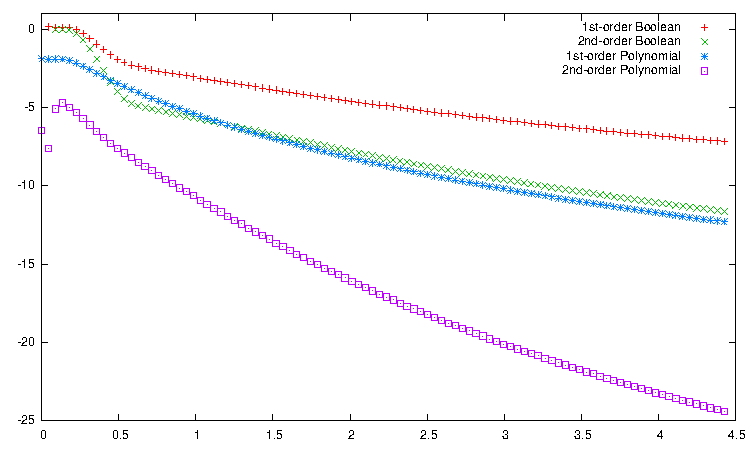
\includegraphics[width=0.7\textwidth]{Figure/mutinf_comparizon.pdf}
\caption{Mutual information (log10) between the leakage and the sensitive variable over
an increasing noise standard deviation (x-axis).}
\label{fig:miBoolSSS}
\end{center}
\end{figure}

\subsubsection{Contributions.} All previous works assume that the most efficient way to attack an $(\nbShares,\order)$-sharing (namely an SSS sharing with $\nbShares$ shares and a degree-$\order$ polynomial) is to observe exactly $\order +1$ shares. The underlying remarks are that (1) observing strictly less shares does not provide information on the shared variable (by property of SSS) and (2) observing strictly more than $\order +1$ shares will merely provide the attacker with more noise than information since the knowledge of exactly $\order +1$ is sufficient to rebuild $\vShared$ (by interpolation). This paper essentially aims at coming back on the second point which has been assumed, without being proved, in all previous works studying SSS in the SCA context. We actually highlight an important difference between Boolean and SSS sharings which implies that, for some signal-to-noise ratio, it is more advantageous for the adversary to observe strictly more than $\order+1$ shares. This is illustrated in the following simulations results which are discussed in Section ...
 \todo{}

It may be observed in Fig. \ref{} that for a noise standard deviation $\sigma \in \{\}$, it is more interesting for the adversary to target ... shares instead of ....  Recent works (see \eg \cite{BCPZ16} and \cite{}) have indeed argued that several manipulations of the same share could be used to improve the efficiency of attacks exploiting only $\order +1$ shares to defeat a $\order$-secure masking. But they cannot explain the important difference observed in Figure \ref{}. Actually, as it will be discussed in this paper the rebuilding of a value $\vShared\in \GFm$ shared with an $(\nbShares,\order)$-SSS sharing may need strictly (much) less than $(\order+1) \times \dimension$ (while it is clear that exactly $(\order + 1)\times \dimension$ bits for information must be recovered in the Boolean case). This implies in particular that it may be more efficient to extract strictly less than $\dimension$ bits of information on $\order'<\order +1$ shares, than to extract $\dimension$ bits of information on exactly $\order + 1$ shares. 

\subsubsection{Paper Outline.}


\section{Preliminaries on Shamir's Secret Sharing.}

In a seminal paper\,\cite{Sha79}, Shamir proposed to split a secret $A\in \GFn$ into $\nbShares$ shares such that
no tuple of shares with cardinality lower than a so-called {\em threshold} $\order<\nbShares$ depends on $A$. Shamir's
protocol consists in associating $A$ with a random polynomial $P_A(X)\doteq A + \sum_{i=1}^{\order}\polyCoef X^i$ of degree lower than $\order$ and with constant term $A=P_A(0)$. Then, the polynomial $P_A(X)$ is evaluated in $\nbShares$ distinct public non-zero elements $\pubElt[0], \ldots, \pubElt[n-1]$ in $\GFn$ to define a so-called {\em $(\nbShares,\order)$-sharing} $(A_0,A_1,\cdots,A_{\nbShares-1})$ of $A$ such that $(A_i)_{i\leqslant \nbShares}=(P_A(\alpha_i))_{i\leqslant \nbShares}$. To re-construct $A$ from its sharing, polynomial interpolation is first applied to re-construct the polynomial from its $\nbShares$ evaluations $A_i$ and then, it is evaluated in $0$. Actually, using Lagrange's
interpolation formula, the two steps can be combined in a single one thanks to the equality $ A=\sum_{i=0}^{\nbShares-1} A_i \cdot \beta_i\enspace$,  where the (public) constants $\beta_i$ are defined as $\beta_i:=\prod_{k=0,k\neq i}^{\nbShares-1} \frac{\alpha_k}{\alpha_i+\alpha_k}$. The vector composed of the $n$ weights $\beta_i$ is denoted by $\vec \beta$ and the scalar product is called $n$-reconstruction. As initially observed by McEliece and Sarwate in \cite{MS81}, the sharing of $A$ described above may be viewed as an {\em encoding} with a Reed-Solomon code of parameters $[\nbShares + 1,\order + 1]$:
$$
(A,A_1,\cdots,A_{\nbShares}) = (A,\polyCoef[1],\cdots,\polyCoef[\order])\times 
\left(\begin{matrix}
1 & 1 & \hdots & 1 \\
0 & \pubElt[1] & \hdots & \pubElt[\nbShares] \\
0 & \pubElt[1]^2 & \hdots & \pubElt[\nbShares]^2 \\
\vdots & \vdots & \hdots & \vdots \\
0 & \pubElt[1]^{\order} & \hdots & \pubElt[\nbShares]^{\order} 
\end{matrix}
\right)
$$
The reconstruction of $A$ then corresponds to a simple {\em decoding}.
\vspace{3mm}

To define a $\order$\myth-order masking scheme for a block cipher
implementation where each intermediate result is split with Shamir's
technique, one must specify a secure method for the processing of field
multiplications over $\GFn$. Most of (if not all) existing protocols start from a multiplication scheme introduced by
Ben-Or \etal in the context of the Multy-Party Computation Theory
\cite{BGW88}. For this protocol to work, the number of shares $\nbShares$ per variable must be at least $2\order+1$ and for $\nbShares=2\order+1$, it is proved that it satisfies a security property encompassing the $\order$\myth-order SCA security \cite{PR11}. We give hereafter the adaptation of
\cite{BGW88} in the 
SCA context as proposed in \cite{PR11,RP12}\footnote{The protocol is 
an improved version of the protocol originally proposed by Ben-Or \etal \cite{BGW88},
due to Gennaro \etal in \cite{GRR98}.}.


\begin{algorithm}
\caption{Secure Multiplication For Shamir's Secret Sharing}
\label{alg:secmult}
\begin{algorithmic}[1]
\Require {two integers $\nbShares$ and $\order$ such that $n\geq 2d+1$, the  $(\nbShares,\order)$-sharings $(u_i)_i=(P_u(\pubElt))_i$ and $(v_i)_i=(P_{v}(\pubElt))_i$ of $u$ and $v$ respectively.}
\Require   {the $\nbShares$ distinct points $\pubElt$, the interpolation values $(\beta_0,\cdots,\beta_{\nbShares-1})$}
\Ensure     {the $(\nbShares,\order)$-sharing $(P_{C}(\alpha_i))_i$ of $w=u\cdot v$. }


\Comment{Compute a $\nbShares$-sharing $(t_1,\cdots,t_n)$ of $w$}
\For{$i=1$ \textbf{to} $\nbShares$}
\State $t_i \leftarrow P_u(\pubElt)\cdot P_{v}(\pubElt)$
\EndFor

\Comment{For every share $t_i$, compute a sharing $(Q_i(\alpha_j))_{j\leq n}$ with $Q_i (X)$ a random degree-$d$ polynomial with constant term $t_i$}
\For{$i=1$ \textbf{to} $\nbShares$}
\For{$j=1$ \textbf{to} $\order$}
\State $\omega_j \leftarrow \texttt{rand}(\GFn)$
\EndFor
\For{$j=1$ \textbf{to} $\nbShares$}
\State $Q_i(\pubElt[j]) \leftarrow \beta_i \cdot t_i +
      \sum_{k=1}^{\order} \omega_k\cdot \pubElt[j]^k$ \label{step:reshare}   	
\EndFor  	
\EndFor
   	
\Comment{Compute the share $w_i = P_{w}(\pubElt)$ for $w=u \cdot v$}
\For{$i=1$ \textbf{to} $\nbShares$}
\State $w_i \leftarrow \sum_{j=1}^{\nbShares} Q_j(\pubElt)$
\EndFor
\Return $(w_i)_i$
\end{algorithmic}
\end{algorithm}



The completeness of Algorithm \ref{alg:secmult} is discussed in \cite{BGW88}. Its $\order$\myth-order SCA security can be straightforwardly deduced from the proof given by Ben-Or \etal in \cite{BGW88} in the secure multi-party computation context. Eventually, for $\nbShares=2\order+1$ (which is the parameter choice which optimizes the security/efficiency overhead), the complexity of Algorithm \ref{alg:secmult} in terms of additions and multiplications is ${\cal O}(\order^3)$.

Algorithm \ref{alg:secmult} may be rewritten in terms of coding theory, essentially because an $(\nbShares,\order)$-sharing with Shamir's scheme exactly corresponds to an encoding by a Reed-Solomon code with parameters $[\nbShares+1,\order+1]$ \cite{MS81}. Let $\RSCode$ denote the latter code and let $\RSProduct$ denote the {\em product code} built from $\RSCode$ by taking all the componentwise products of codewords in $\RSCode$. On one hand, the tuple $\wordRSProduct = (t_1,\cdots,t_{2n})$ in Algorithm \ref{alg:secmult} forms a sharing of $w=u\cdot v$ in $\RSProduct$ and a reconstruction algorithm is simply given by the scalar product with $\vec \beta$ (this is a direct consequence of Lagrange's interpolation formula). On the other hand, loop $6$-$8$ (over indices $i$ and $j$) and loop $10$-$12$ may be viewed as a {\em transcoding} $\trans$ that securely transforms the sharing $\wordRSProduct\in \RSProduct$ of $w$  into a sharing $\wordRS \in \RSCode$. Eventually, it can be observed that the algorithm completeness holds because the constant term of the polynomial associated to the codeword $\RSCode$ has constant term the $n$-reconstruction $\sum_i \beta_i\cdot w_i$. If the product by $\beta_i$ is done once during the building of $t_i$ (at Step $2$), then Algorithm \ref{alg:secmult} involves $n$ multiplications and the evaluations of $\nbShares$ degree-$d$ polynomials in $n$ points (which makes $\nbShares^2\times d$ multiplications for a naive implementation and $O(\nbShares \log^2 \nbShares)$ multiplications using FFT-based polynomial division\footnote{The constant terms being important in this complexity the naive approach is always more efficient for practical choices of $\nbShares$ and $\order$.} \cite{CPR12}). In \cite{CRZ13}, the authors observed that the addition of a random sharing $\wordRSProductZero\in \RSProduct$ of $0$ to $\wordRSProduct$ makes it possible to reduce the number of polynomials to evaluate from $\nbShares$ to $\order+1$, without compromising the security at order $\order$. The core idea is to precede the transcoding by a shortening of the sharing $\wordRSNew \doteq (\wordRSProduct_1 + \wordRSProductZero_1,\cdots,\wordRSProduct_{\nbShares} + \wordRSProductZero_{\nbShares} )$ into $(\sum_{i=1}^{\nbShares - \order}\beta_i \wordRSNew_i,\beta_{\nbShares -\order+1}\wordRSNew_{\nbShares -\order+1},\cdots,\beta_{\nbShares}\wordRSNew_{\nbShares})$.





\section{Side-Channel analysis of Shamir's Secret Sharing Scheme}
\subsection{Higher-order Side-Channel Resistance: Requirements and Limitations}
\subsubsection{Higher-order Side-Channel Resistance: Requirements.} To design a $\order$\myth-order masking scheme based on Shamir's Secret Sharing for a block cipher, one have to develop some procedures to protect the different operations involved in this protected algorithm. For instance, most of (if not all) linear operations (\emph{e.g.} XOR) are compatible with linear secret sharing. However, nonlinear operations (\emph{e.g.} AES SBox) are more difficult to deal with since it require to protect the multiplication of shares. Some solutions have been developed in the context of protecting the AES using the Shamir's Secret Sharing\cite{GM11,PR11,RP12} and are mainly based on the multiplication scheme introduced by
Ben-Or \etal to design secure multy-party computation schemes\cite{BGW88}.
The method is described in \ref{alg:secmult} and consists in multiplying each two share vectors share by share. This operation corresponds to the multiplication of two degree $d$ polynomials which gives a polynomial of degree $2d$. The secret result of the multiplication can then be recovered with at least $2d + 1$ shares if $n > 2t + 1$. 
So, to achieve a $\order$\myth-order resistance against side-channel attack, the sharing order must be at least $n = 2d + 1$ (\emph{i.e.} the smallest value allowed in Ben-Or \etal multiplication protocol to guarantee $d$\myth-order resistance).

\subsubsection{Higher-order Side-Channel Resistance: Limitations.} On the other hand, a Shamir's secret sharing scheme is said to be secure at the $d$\myth-order if any set of at most $d$ shares reveals no information about the shared secret value. 

\begin{remark}
From an attacker perspective, given an $(n=2d+1,d)$ secret sharing it is theoretically possible to recover the shared secret value by exploiting the leakage of any $(d+1)$ combination of shares over the $d+1 \choose n=2d+1$ possible ones. 
\label{rmk:sca}
\end{remark}
\subsubsection{Higher-order Side-Channel Attack Effectiveness: Discussions.} 
Based on Remark~\ref{rmk:sca}, the following questions would be investigated:
\begin{enumerate}
\item \emph{did all $(d+1)$ combination of shares achieve the same attack efficiency?} Actually, an attacker is spoilt for the choice of the combination of $d+1$ shares to use among the several available ones. Our goal here is to check if all $d+1$ combination of shares leak the same amount of information under the same fixed noise level for each share. The result of this investigation may brings some insights on the optimal $(d+1)$ combination of shares, if any exits, that an attacker should consider when performing his attack.

\item \emph{Did any $(d+2)$ combination of shares achieves a better attack result than all $(d+1)$ combination of shares?}. This question is motivated by the fact that when exploiting the leakage of $(d+2)$ combination of shares, the attacker have theoretically access to exactly the same amount of information leaked by any $(d+1)$ combination of shares. Our purpose here is to check the effectiveness of this claim. If the use of some $(d+2)$ combination of shares are more optimal than some (or all) $(d+1)$ combination of shares in terms of side-channel attack efficiency to recover the  secret value, then one can conclude that the shares are not leaking the same amount of information.
\end{enumerate}    

In what follows, we try to answer these questions by performing practical attacks on simulated traces and real acquisitions captured on the ChipWhisperer platform~\cite{O’Flynn2014}.

\subsection{Attack results on Simulated Traces}
\subsubsection{Target Implementation.}
For our simulation, we targeted a $(5,2)$ secret sharing scheme, \emph{i.e.} the secret value $Z \in GF(2^8)$ is split into $5$ independent shares $(S_0, \cdots, S_4)$ by evaluating a random polynomial of degree $2$ ($P_Z(X)= Z + \mu_1 X + \mu_2 X^2$) in $5$ public points $(\alpha_0, \cdots, \alpha_4)$ and where $\mu_1$ and $\mu_2$ are two random values in $GF(2^8)$.    

\subsubsection{Leakage Model.}
During the execution of the algorithm, the processing of each share $S_i$ produces some leakage $L_i$ revealing some information about the share value. In our simulation, we have make the following assumptions:
\begin{itemize}
\item given the values of the shares, the leakage has a Gaussian distribution. This assumption is fairly realistic and commonly used in side-channel context~\cite{LPRRT14}, and formally stated by: 
\begin{equation*}
(L_i | S_i = s) \sim \mathcal{N} (m_{i,s}, \Sigma_{j,s}) \enspace,
\end{equation*}
for every share $i$ and for every $s \in GF(2^8)$, where $m_{i,s}$ are expectation vectors defined over $\mathbb{R}^T$ and $\Sigma_{j,s}$ are covariance matrices defined over $\mathbb{R}^{T \times T}$ with $T$ is the dimension of the leakage for each share and is set at $T=1$ in our simulation setup\footnote{If the dimension $T$ equals $1$, then the Gaussian distribution is said to be univariate and its covariance matrix is reduced to the variance of the single coordinate denoted $\sigma^2$. If the $T$ is greater
than $1$, the Gaussian distribution is said to be multivariate.}.
\item The leakage $L_i$ is the sum of two \textit{mutually independent} parts: a deterministic function $f_i$ of the share $S_i$ and a Gaussian noise $N_i$:
\begin{equation*}
L_i = f_i(S_i) +  N_i \enspace.
\end{equation*}
To generate our traces, we considered two types of functions: the Hamming weight and the identity. 
\item The noises $N_i$ are mutually independent and have the same fixed variance ($\sigma^2$). The rational behind this assumption is to have the same noise level for each share. 
\end{itemize}

\subsubsection{Attack Strategy.} To evaluate the $(5,2)$ secret sharing, we have performed a higher-order template attack following the procedure described in~\cite{LPRRT14}. Let $(\boldsymbol{\ell_i})_{1\le i \le N} \in \mathbb{R}^5$ be the set of collected traces for the attack phase, then for any key hypothesis value $k\in GF(2^8)$, the likelihood distinguisher\footnote{In practice, one often makes use of the equivalent (averaged) log-likelihood distinguisher.} is defined as:

\begin{equation*}
d_k= \prod\limits_{i=1}^{N} p_{k}(\boldsymbol{\ell_i}) \enspace,
\end{equation*}    
 
where $p_k$ denotes the probability density function (pdf) of the leakage. Under the Gaussian assumption, the pdf satisfies:   

\begin{equation}
p_s : (\boldsymbol{\ell_i}) = (\boldsymbol{\ell_{0,i}}, \cdots, \boldsymbol{\ell_{4,i}}) \mapsto \frac{1}{256^5} \sum_{s_1 \in GF(2^8)} \cdots \sum_{s_4 \in GF(2^8)} \prod\limits_{j=0}^{4} \phi_{m_{j,s_j}, \sigma^2} (\boldsymbol{\ell_{j,i}})
\label{eq_pdf}
\end{equation} 
 
where, for every value $x \in \mathbb{R}$, the function $\phi_{m,\sigma^2}(x)$ denotes the pdf of a Gaussian distribution with a mean equals to $m$ and a variance equals to $\sigma^2$. 

In~\cite{LPRRT14} authors have demonstrated that for a $d$\myth-order Boolean masking \eqref{eq_pdf} can be expressed as a higher-order convolution product and then they have provided an efficient method to evaluate this formula in $ \mathcal{O}(d \cdot |GF(2^8)| \cdot log|GF(2^8)|)$ operations. 
We recall that:
\begin{itemize}
\item  when a $d$\myth-order Boolean masking is applied, we have $s_0= Z \oplus \bigoplus\limits_{i=1}^{d} (s_i)$ where the $(s_i)_{1 \le i \le d}$ here denotes the random masks.

\item When a $(n,d)$ secret sharing is applied, the sensitive variable $Z$ stratifies: 
\begin{equation}
Z=\bigoplus\limits_{i=0}^{d} (s_i \cdot \beta_i) \enspace,
\label{eq_Z}
\end{equation}
 where $s_i =P_Z(\alpha_i)$ and $\beta_i=\prod\limits_{k=0,k\neq i}^{d} \frac{\alpha_k}{\alpha_i+\alpha_k}$. 
\end{itemize}

To continue using the efficient procedure for higher-order pdf estimation proposed in~\cite{LPRRT14} in the context of secret sharing scheme, we propose hereafter a simple trick. In fact, we can rewrite \eqref{eq_Z} as $s_0=\frac{Z}{\beta_0}\oplus\bigoplus\limits_{i=1}^{d} (s_i \cdot \frac{\beta_i}{\beta_0})$ and then by denoting $Z'=\frac{Z}{\beta_0}$ and $s'=s_i \cdot \frac{\beta_i}{\beta_0}$ for every $i \in [ 1: d$ we obtain:

\begin{equation*}
s_0= Z' \oplus \bigoplus\limits_{i=1}^{d} (s'_i) \enspace.
\end{equation*}

So to evaluate the $(5,2)$ secret sharing scheme, our methodology consists of two-steps:

\begin{enumerate}
\item Profile the leakage of every share using standard estimation techniques. Under the Gaussian leakage assumption, this estimation amounts to compute the sample means ($m_{i,s_i}$) and variance ($\sigma^2$) of the leakage $(L_i | S_i = s)$ for every share $S_i$ and every possible value $s_i$ based on a set of collected leakage samples.
\item Use \label{eq_pdf} to perform the higher-order template attack on a new set of collected traces generated with an unknown secret value $Z$.
\end{enumerate} 

\subsubsection{Attack Results.} 

We plot in Fig.~\ref{fig_3_shares}, for each possible combination of $3$ shares the evolution of the number of traces required to achieve $100\%$ of success rate according to an increasing noise standard deviation. We stress the fact that for each value of the standard deviation, the attacks have been repeated $1.000$ times.  

\begin{figure}
\begin{center}
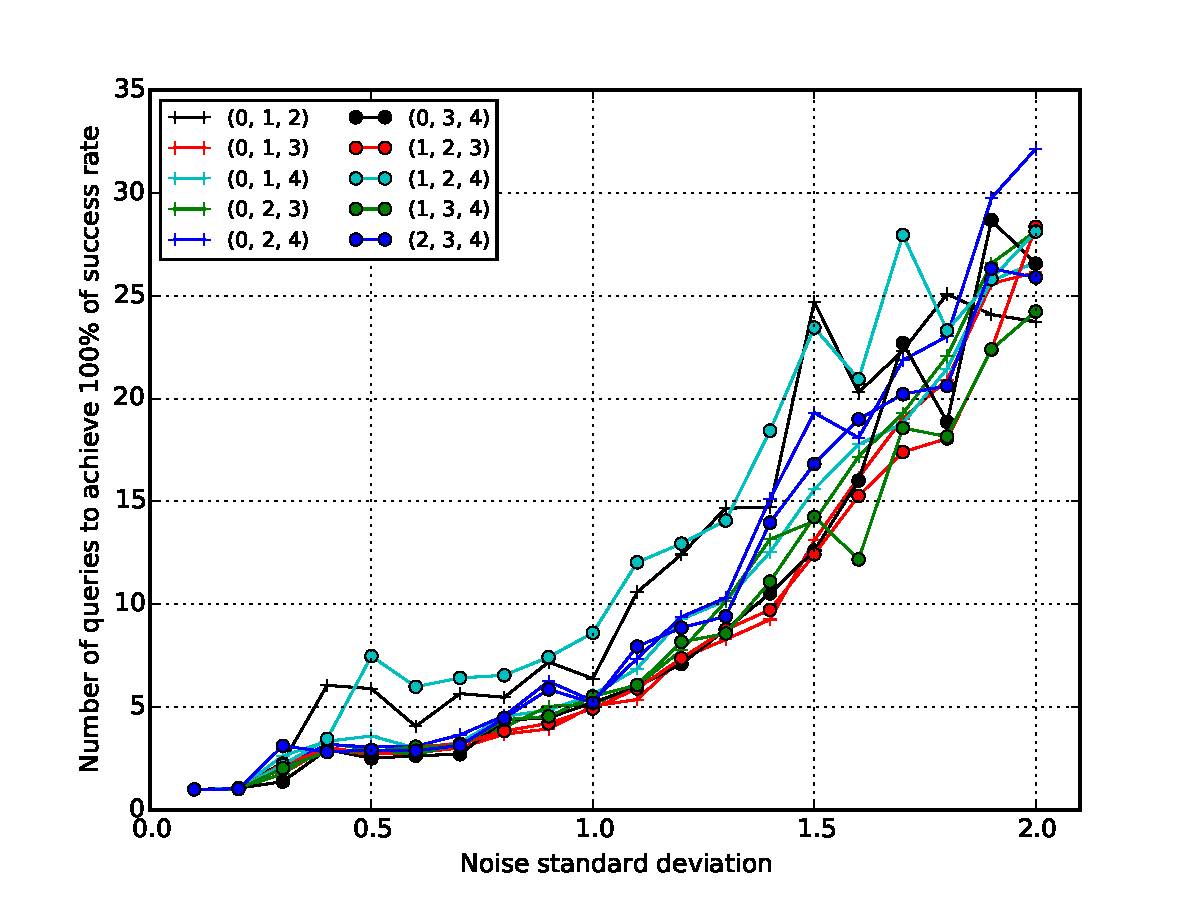
\includegraphics[width=1\textwidth]{Figure/res_125_246_119_104_150.pdf}
\caption{Evolution of the number of queries to achieve $100\%$ of success rate according to an increasing noise standard deviation.}
\label{fig_3_shares}
\end{center}
\end{figure}

From Fig.~\ref{fig_3_shares}, we observe that some combinations of $3$-shares perform worst than others despite the fact that all shares have the same level of noise. This result could be explained by the fact that the amount of information is different for each share. Hence, an attacker have to choose the optimal combination of $3$ shares to succeed his attack with less traces. Indeed, we have observed that when we use another set of public points the attack results are different and the optimal combinations of $3$-shares change too as shown in Fig.~\ref{fig_3_shares_bis}.    

\begin{figure}
\begin{center}
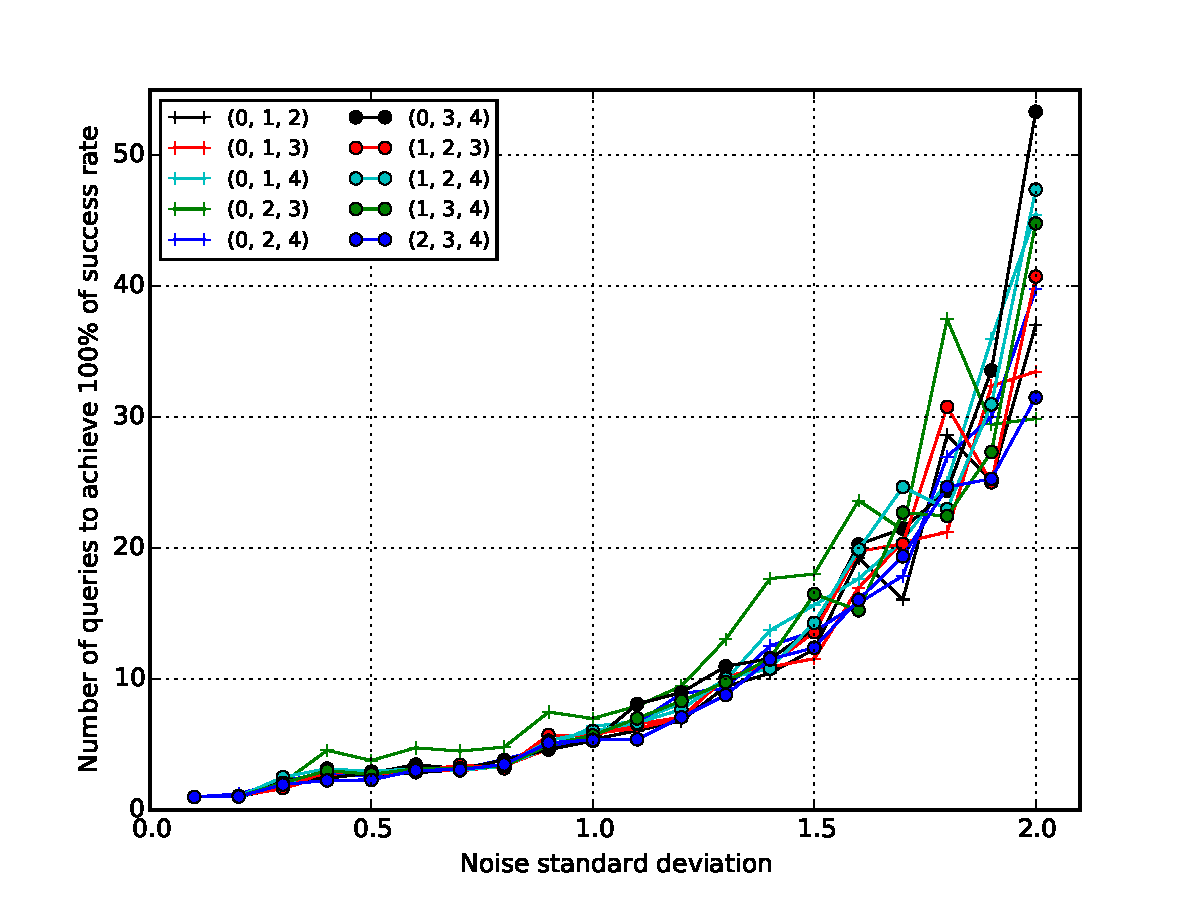
\includegraphics[width=1\textwidth]{Figure/res_86_23_115_107_189.pdf}
\caption{Evolution of the number of queries to achieve $100\%$ of success rate according to an increasing noise standard deviation.}
\label{fig_3_shares_bis}
\end{center}
\end{figure}

Based on these results, we answer the question (did all $(d+1)$ combination of shares achieve the same attack efficiency?) negatively.

The second investigation we planned to perform is to check if exploiting the leakage of $4$ shares could be more efficient than some or all combination of $3$ shares. We show in Fig.~\ref{fig_4_shares} a comparison between the template attack results when considering all combination of $3$ and $4$ shares. The experiences are repeated $1.000$ times for each combination of shares.

\begin{figure}
\begin{center}
%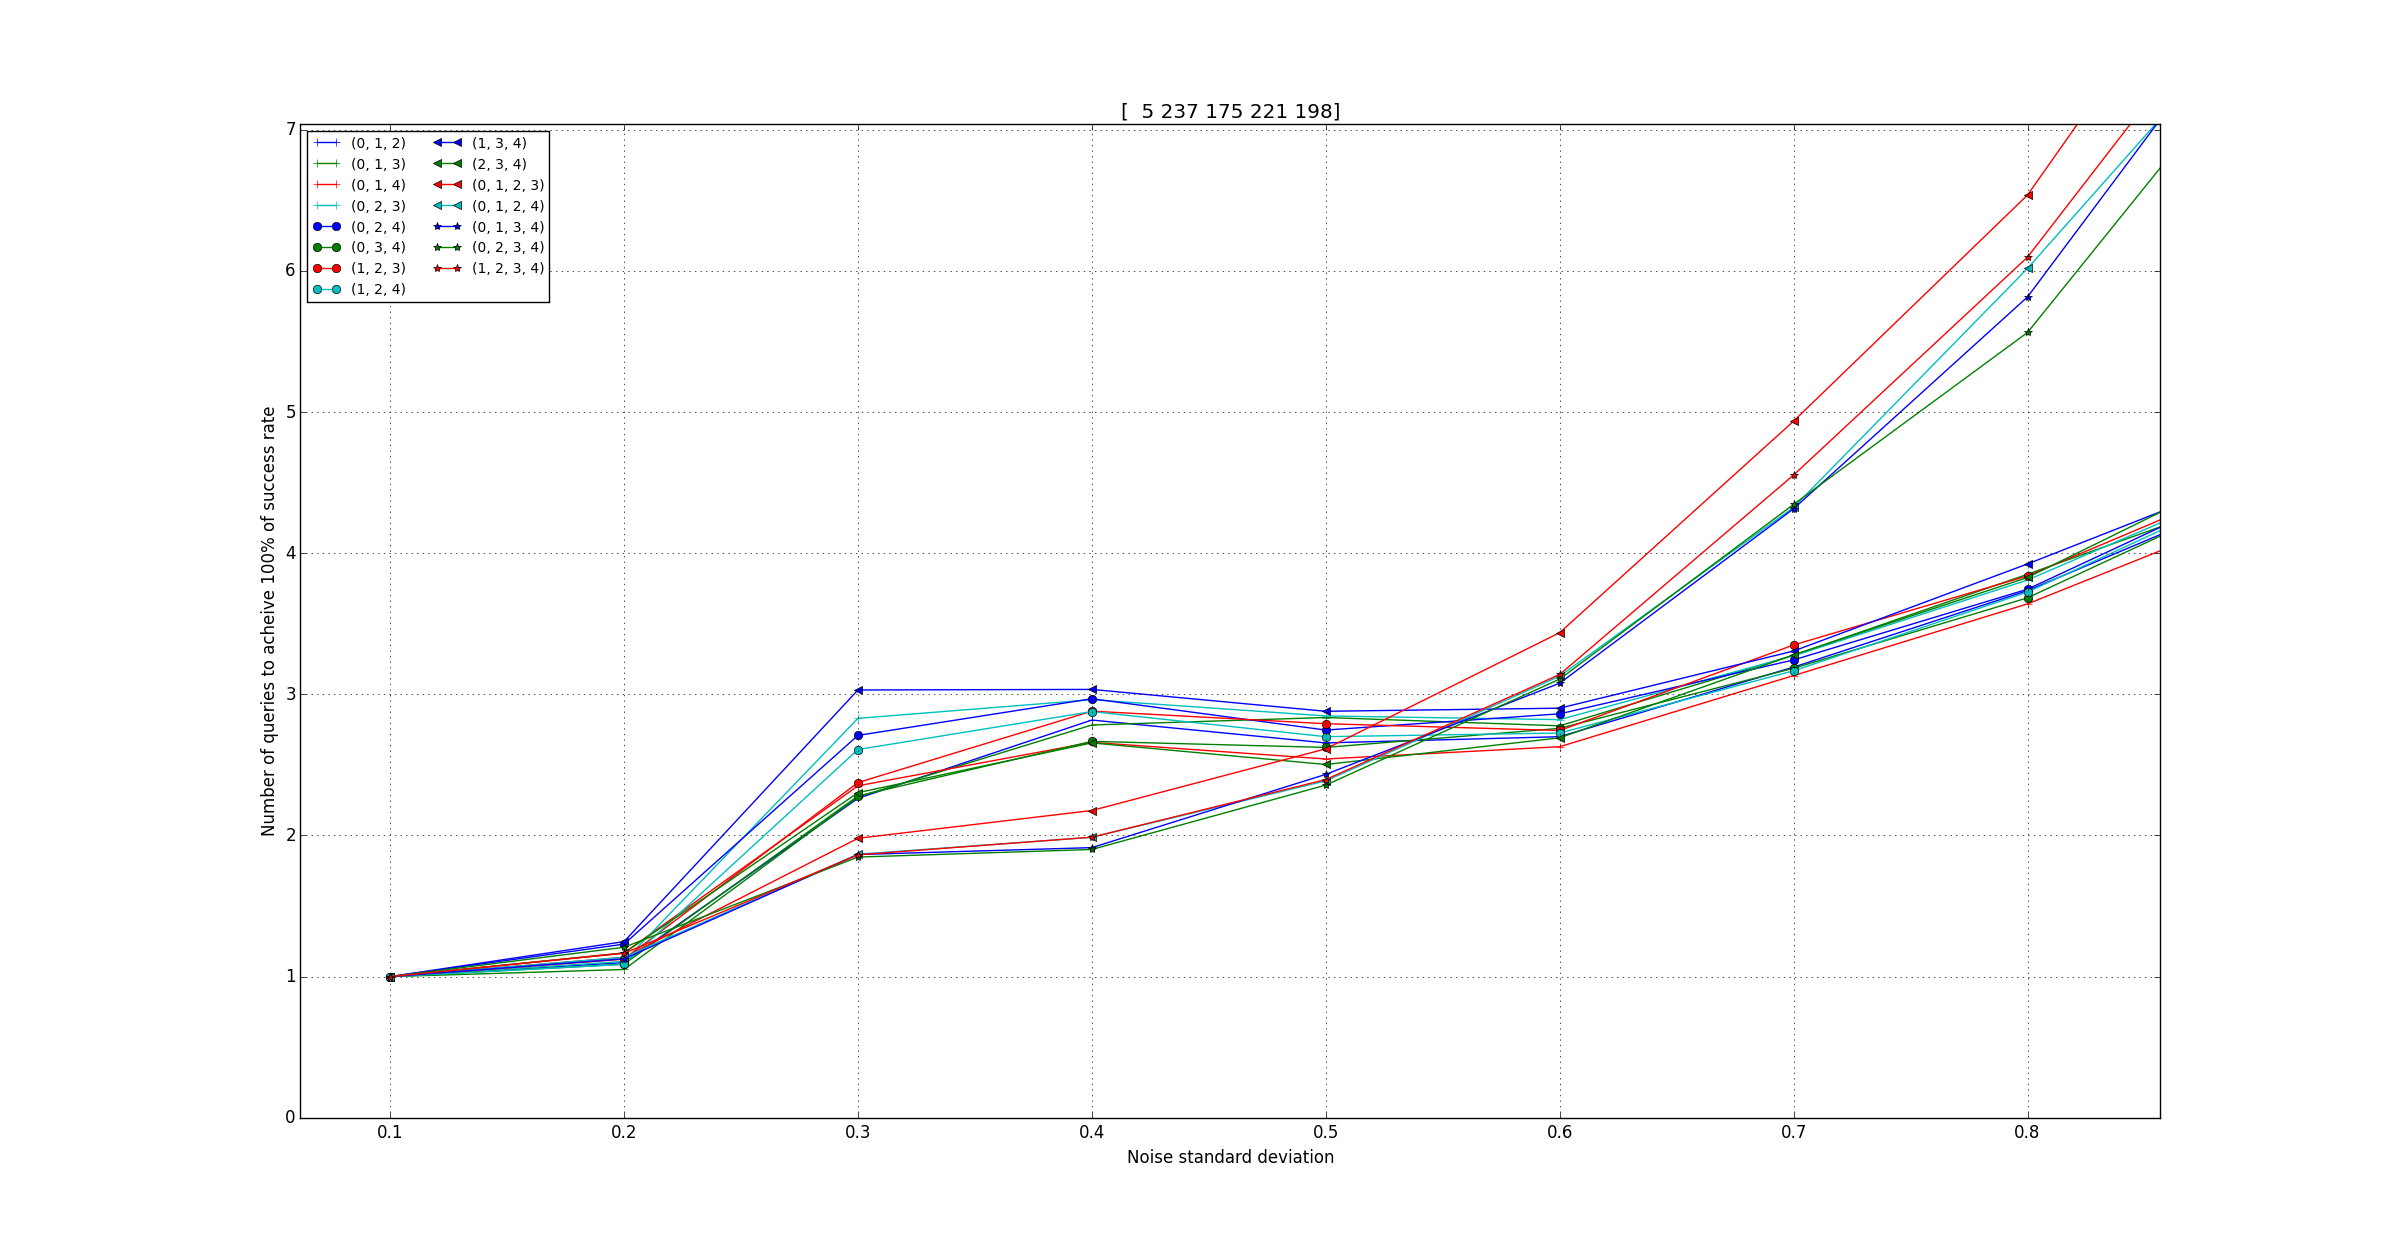
\includegraphics[width=1\textwidth]{Figure/5_237_zoom.pdf}
\caption{Evolution of the number of queries to achieve $100\%$ of success rate according to an increasing noise standard deviation.}
\label{fig_4_shares}
\end{center}
\end{figure}

From Fig.~\ref{fig_4_shares}, one can identify that for a specific interval of noise standard deviation, some combination of $4$ outperform all or some combination of $3$ shares. The same observation is valid when changing the set of public points as described in Fig.~\ref{fig_4_shares_bis}.

\begin{figure}
\begin{center}
%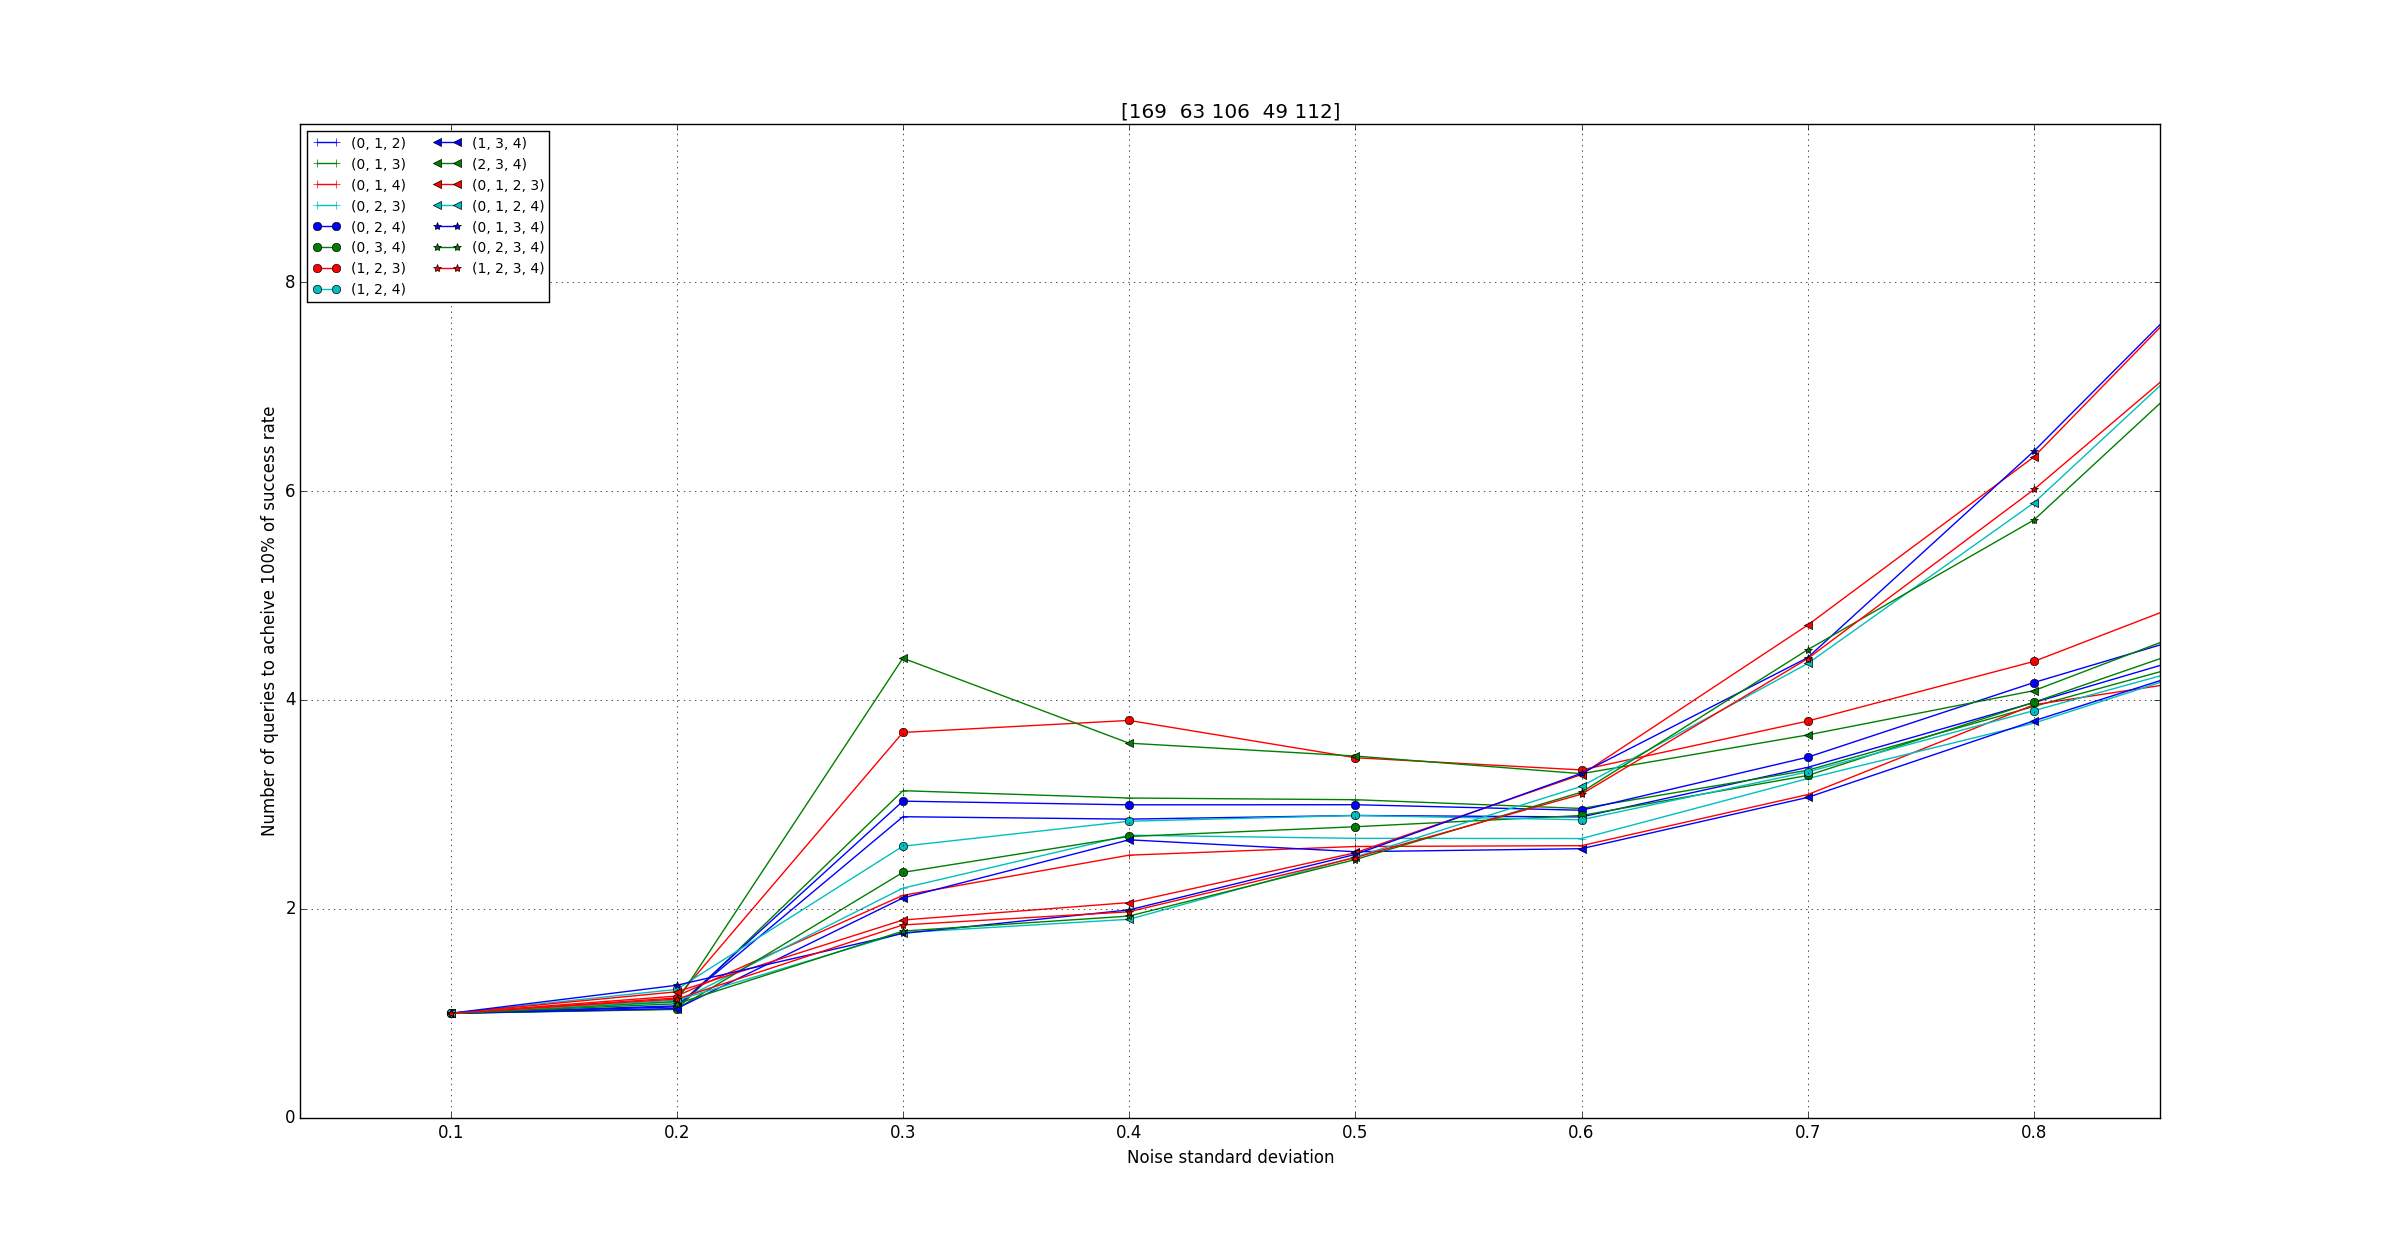
\includegraphics[width=1\textwidth]{Figure/169_63_zoom.pdf}
\caption{Evolution of the number of queries to achieve $100\%$ of success rate according to an increasing noise standard deviation.}
\label{fig_4_shares_bis}
\end{center}
\end{figure}

From Fig.~\ref{fig_4_shares} and Fig.~\ref{fig_4_shares_bis}, the following observations could be emphasized:

\begin{itemize}
\item The shares are not leaking the same amount of leakage despite the fact that the same quantity of noise has been added to the $5$ used shares to protect the sensitive value $Z$. one can easily notice the differences in terms of attack efficiency when comparing the different used combinations of $4$ and $3$ shares.
\item Exploiting the leakage of $4$ shares is more efficient than all combination of $3$ shares for some values of the noise standard deviation. This result could be explained by the fact that the combination of $4$ shares may exploit less amount of information from the leaking shares (than all combination of $3$ shares) to recover efficiently (and fast) the secret value (\emph{i.e.} with less traces). When the noise increases, the efficiency of the template attacks exploiting $4$ shares decreases with respect to these using combination of $3$ shares. This behavior is expected since the more noisy shares you combine, the less the signal-to-noise-ration is. 
\item When comparing both Fig.~\ref{fig_4_shares} and Fig.~\ref{fig_4_shares_bis}, one can notice that the optimal combination of $4$ shares to recover the secret value changes with respect to the used public points. So, the amount of information leaked by the shares depend on the set of public points used to share the secret value. Therefore, an attacker has to adapt the choice of shares to use for his attack with respect to the used set of public points.
\end{itemize}

Based on these observations, we answer the question (Did any $(d+2)$ combination of shares achieves a better attack result than all $(d+1)$ combination of shares?) positively. 

In order to confirm our findings on simulated traces, we conducted some practical attacks on the ChipWhisperer platform. The experimental setup is described in what follows. 

\subsection{Attack results on Real Device}

First, we have implemented a $(5,2)$ secret sharing on an $8$-bit AVR microprocessor atxmega128d3 and we acquired power-consumption traces thanks to the ChipWhisperer-Lite (CW1173) basic board. For the leakage profiling step, we have collected $128.000$ traces to estimate the mean and the variance for each share. These statistical estimation results have shown that the shares have roughly the same variance (\emph{i.e.} the same level of noise) which is in-line with our simulation setup. However, the standard deviation of the noise of the acquired traces is actually outside the suitable area where the combinations of $4$ shares outperform the combination of $3$ shares. The estimated noise standard deviation is about $0.7$.
Then, we have acquired $15.000$ traces for the attack phase and we have performed the template attack by exploiting the leakage of all combination of $4$ and $3$ shares. As expected, the attack results have demonstrated that any combinations of $4$ shares is efficient with respect to the measures noise standard deviation. To decrease the noise level and to fit the suitable interval, we filtered the acquired traces to reach a noise standard deviation value equal to $0.5$. Finally, we re-performed our higher-order template attack. The success rate of the attack for each combination of share is shown in Fig.~\ref{fig_4_shares}.    

\begin{figure}
\begin{center}
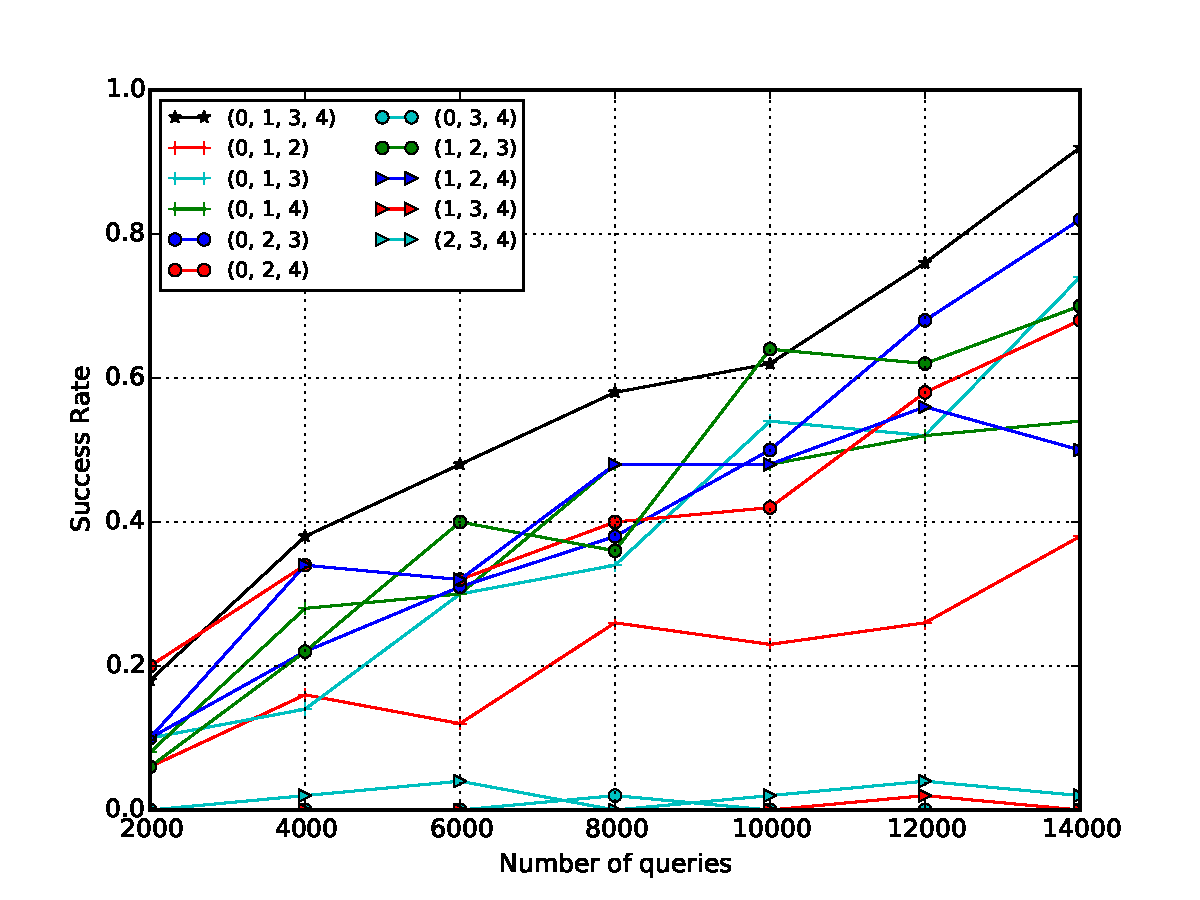
\includegraphics[width=1\textwidth]{Figure/SR.pdf}
\caption{Success rate of the template attack according to an increasing number of traces.}
\label{fig_SR}
\end{center}
\end{figure}

From Fig.~\ref{fig_SR}, one can see that exploiting the leakage of the shares $(0, 1, 3, 4)$ is more suitable in terms of attack efficiency since we require less power measurements to achieve $90\%$ of success rate compared to all combination of $3$ shares. 



\section{Improvement Proposal of Shamir's Secret Sharing Scheme}

\subsection{Linear Exact Repairing Codes}

A {\em linear code} $\mathcal{C}$ of length $\nbShares$ and dimension $k$ over a finite field $\Field$ is a $k$-dimensional subspace of $\Field^{\nbShares}$. It is denoted by $\mathcal{C}[n,k]$. A particular linear code is the {\em Reed-Solomon Code} whose definition is recalled hereafter.

\begin{definition}[Reed-Solomon Code]
The Reed-Solomon code $\RS[\pubSet, \order + 1]\subseteq \Field^{\nbShares}$ of dimension $\order + 1$ over a finite field $\Field$ and with evaluation subset $\pubSet = \{\pubElt[1],\pubElt[2],\cdots,\pubElt[\nbShares]\}$ of $\Field$ is the subspace:
$$\RS[\pubSet,\order + 1] = \{(P(\pubElt[1]),P(\pubElt[2]),\cdots,P(\pubElt[\nbShares])); P(X) \in \Field[X] \text{ and } \deg(P) \leqslant \order\} \enspace .$$
\end{definition}

Reed-Solomon codes are {\em Maximum Distance Separable} (MDS) codes, which means that any $\order + 1$ symbols (that is, evaluations of a polynomial $P(X)\in \RS[\pubSet,\order+1]$) can be used to recover the entire codeword (that is,
$P(X)$ itself).
\vspace{3mm}

Let us assume that a file, consisting of $\order + 1$ blocks, is encoded into $\nbShares$ nodes. {\em Exact Repairing codes} have been originally introduced to recover the contents of an erased node by downloading some information from the remaining nodes. In the language of an $\RS[\pubSet,\order+1]$ code as above, the file is a polynomial $P(X)\in \Field[X]$ with $\deg(P(X)) \leqslant \order$ and each node is associated with an evaluation point $\pubElt \in \pubSet$ and stores $P(\pubElt)$. For an arbitrary $\pubEltStar\in \pubSet$ (corresponding to an erased node), the goal is to recover $P(\pubEltStar)$ given some information from the other nodes. Since the code is MDS, its is straightforward to do it by choosing any subset of $\pubSet$ with cardinality $\order + 1$ and by asking the evaluations $P(\pubElt)$ to the corresponding nodes. This means that, for any $\pubEltStar$, the evaluation $P(\pubEltStar)$ can at least be recovered by asking $\log_2(\Field)$ bits of information (corresponding to $P(\pubElt)$) to $\order +1$ nodes. Linear repairing codes aim to define a repairing scheme such that, for any $\pubEltStar$, the evaluation $P(\pubEltStar)$ can be recovered with strictly less than $(\order + 1)\times \log_2(\Field)$ bits of information, by allowing each node to return any $\FField$-linear function of its content, with $\FField$ being a subfield of $\Field$. The $\FField$-linear functions from $\FField$ to $\Field$ may all be defined from the so-called {\em field trace} of $\Field$ over $\FField$. We recall the definition of the field trace hereafter:

\begin{definition}[Field Trace]
Let $p$ and $r$ be two integers and let $q=p^r$. Let $\Field=\GF(q^t)$ be a degree-$t$ finite field extension of a $\FField=\GF(q)$. The {\em field trace} $\myTrace$ is defined for every $\beta \in \Field$ as:
\begin{equation}\label{equ:trace}
\myTrace(\beta) = \beta + \beta^q + \beta^{q^2} + \cdots + \beta^{q^{t-1}} \enspace .
\end{equation}
\end{definition}

In a linear repair scheme, the node corresponding to a public point $\pubElt$ returns zero or more elements of $\FField$ of the form $\myTrace(\gamma P(\pubElt))$ for some field elements $\gamma \in \Field$. A linear exact repair scheme can then be described by the field elements $\gamma$ used by all the nodes, along with a (linear) repair algorithm. A precise definition in the context of Reed-Solomon codes is given below:

\begin{definition}[Linear Exact Repair Scheme (LERS)]\label{def:LERS}
Let $\pubSet = \{\pubElt[1],\pubElt[2],\cdots,\pubElt[\nbShares]\}$ be an evaluation subset of a finite field $\Field$ and let $\RS[\pubSet, \order + 1]\subseteq \Field^{\nbShares}$ be the corresponding Reed-Solomon code. A {\em linear exact repair scheme} for this code over a subfield $\FField$ of $\Field$ is composed of the following steps:
\begin{itemize}
\item for each $\pubEltStar\in \pubSet$, and for each $\pubEltNoIndex\in \pubSet \slash \{\pubEltStar\}$, a set of queries $Q_{\pubEltNoIndex}(\pubEltStar)\subseteq \Field$,
\item for each $\pubEltNoIndex \in \pubSet$ and any polynomial $P(X)\in \Field[X]$ with degree lower than $\order +1$, a linear reconstruction algorithm that computes 
$$
P(\pubEltStar) = \sum_{i=1}^t\lambda_i \cdot \nu_i \enspace ,
$$
for coefficients $\lambda_i\in \FField$ and a basis $\{\nu_1,\nu_2,\cdots,\nu_t\}$ for $\Field$ over $\FField$, so that the coefficients $\lambda_i$ are $\FField$-linear combinations of the queries in 
$$
\bigcup_{\pubEltNoIndex \in \pubSet \slash \{\pubEltStar\}}\{\myTrace(\gamma\cdot P(\pubEltNoIndex); \gamma \in Q_{\pubEltNoIndex}(\pubEltStar)\} \enspace .
$$
\end{itemize}
\end{definition}

The {\em repair bandwith} $RB$ of a LERS is the maximum number of sub-symbols which must be returned by the nodes to recover $P(\pubEltStar)$. It is defined by:
$$
RB = \max_{\pubEltStar \in \pubSet} \sum_{\pubEltNoIndex \in \pubSet \slash \{\pubEltStar\}} \# Q_{\pubEltNoIndex}(\pubEltStar) \enspace .
$$

One of the main goals of LERS schemes is to minimize the maximum number of bits $RB\times \log_2(\FField)$ required to reconstruct $P(\pubEltStar)$ for any $\pubEltStar\in \pubSet$ and any polynomial $P(X)$. During the last few years, there have been several publications tackling this issue in the context of RS codes (see \eg \cite{DRWS11,SPDC13}), or more generally, for MDS codes (see \eg \cite{CHJL11,DGWWR10,SR10}). Depending on the extension dimension $t$ of $\Field$ over $\FField$, some lower bounds have been given:
\begin{itemize}
\item when $t$ is sufficiently large, $RB$ is bounded below by $(t\cdot RL)/(RL-\order)$, where $RL$ denotes the {\em repair locality} and corresponds to the maximum number of $\pubElt \in \pubSet$ that are required to recover $P(\pubEltStar)$ whatever $\pubEltStar \in \pubSet$. For very large values of $t$, several schemes have been proposed for which the lower bound is achieved (see \eg \cite{CHJL11,SR10}).
\item when $t$ is small, it is clear that the lower bound above cannot be achieved since we have $RB \geqslant \order + t$. It must however be observed that this latter bound is much better than the naive one $t\times (\order + 1)$. \comEP{To continue...}
\end{itemize}
\subsection{Explicit Constructions for Reed-Solomon Codes}
In the recent work \cite{GW16}, the authors show that the construction of a LERS for a Reed-Solomon code $\RS[\pubSet, \order + 1]$ and a subfield $\FField$ of $\Field$
is equivalent to the finding, for any $\pubEltStar\in \pubSet$, of field elements $(\zeta_j)_{j\leqslant t}$ and $(\mu_{\pubEltNoIndex,\zeta_j}(\pubEltStar))_{j\leqslant t,,\pubEltNoIndex \in \pubSet}$, such that:
\begin{itemize}
\item (1) for any $j\in [1:t]$, we have 
\begin{equation}\label{equ:LERS_1}
\myTrace(\zeta_j P(\pubEltStar)) = \sum_{\pubEltNoIndex \in \pubSet \slash \{\pubEltStar\}} \myTrace(\mu_{\pubEltNoIndex,\zeta_j}(\pubEltStar)P(\pubEltNoIndex))
\end{equation}
\item and (2) the following equality holds
\begin{equation}\label{equ:LERS_2}
P(\pubEltStar) = \sum_{j=1}^t \myTrace(\zeta_j P(\pubEltStar)) \enspace .
\end{equation}
\end{itemize}
The core observation in \cite{GW16} is that, surprisingly, for some $\pubEltNoIndex\in \pubSet$ the size of all the elements required to build the set $\{\myTrace(\zeta_j P(\pubEltNoIndex));j\in [1;t]\}$ may be smaller than $P(\pubEltNoIndex)$. This implies that the total number of bits required to recover $P(\pubEltStar)$ from \eqref{equ:LERS_1} and \eqref{equ:LERS_2} may be smaller than $(\order +1)\log_2(\# \Field)$ (corresponding to a direct polynomial interpolation). Actually, it is shown in \cite{GW16} that the construction of field elements $(\zeta_j)_{j\leqslant t}$ and $(\mu_{\pubEltNoIndex,\zeta_j}(\pubEltStar))_{j\leqslant t,,\pubEltNoIndex \in \pubSet}$ minimizing the repair bandwidth is equivalent to the problem of finding some nice polynomials over $\Field$ \cite[Theorem 4]{GW16} and some explicit constructions are proposed. In the specific case of Reed-Solomon codes $\RS[\pubSet, \order + 1]$, the construction of the coefficients $(\zeta_j)_{j\leqslant t}$ and $(\mu_{\pubEltNoIndex,\zeta_j}(\pubEltStar))_{j\leqslant t,,\pubEltNoIndex \in \pubSet}$ leading to some repair bandwidth $RB$ over a subfield $\FField\subseteq \Field$ such that $t=[\Field:\FField]$ can be directly deduced from a set $\polySet\in \Field[X]$ of $t$ polynomials of degree $\nbShares - \order - 1$ so that:
$$
\dim_{\FField} (\{p(\pubEltStar): p\in \polySet\}) = t
$$
and the sets $\{p(\pubEltNoIndex): p\in \polySet\}$ for $\pubEltNoIndex \neq \pubEltStar$ satisfy:
$$
RB \geqslant \sum_{\pubEltNoIndex \in \pubSet \backslash \{\pubEltStar\}} \dim_{\FField} (\{p(\pubEltNoIndex): p\in \polySet\}) \enspace .
$$
Once such a family of polynomials $\polySet$ is found the coefficients are built so that
$$
\{\zeta_1,\cdots,\zeta_t\} = \{p(\pubEltStar): p\in \polySet\}
$$
and for every $j\in [1:t]$ and $\pubEltNoIndex \in \pubSet \backslash \{\pubEltStar\}$;
$$
\mu_{\pubEltNoIndex,\zeta_j}(\pubEltStar) = p(\pubEltNoIndex)\times \frac{\prod_{\beta\in \pubSet \backslash \{\pubEltStar\}}(\pubEltStar - \beta)}{\prod_{\beta\in \pubSet \backslash \{\pubEltStar\}}(\pubEltNoIndex - \beta)} \enspace .
$$

 
\subsection{Example}
 \todo{}


\section{Conclusion}
\label{sec-conc}
 \todo{}
 
%\bibliographystyle{abbrv}
%\bibliography{sca,ANSSI}



\printbibliography
\end{document}
